\documentclass[12pt,a4paper]{article}
\usepackage{amsmath,amssymb,amsthm,epsf, graphicx, rotating}
\usepackage{fancyhdr}
\usepackage{subfig}
\usepackage{float}
\graphicspath{ {./images/} }

\pagestyle{empty}
\setlength{\parindent}{0pt}
\setlength{\textwidth}{6.5in}
\setlength{\oddsidemargin}{0in}
\addtolength{\textheight}{1in}

\renewcommand\theenumi{\alph{enumi}}
\renewcommand\labelenumi{(\theenumi)}

\newcommand{\Z}{\mathbb{Z}}
\newcommand{\F}{\mathbb{F}}
\newcommand{\R}{\mathbb{R}}
\newcommand{\C}{\mathbb{C}}
\newcommand{\N}{\mathbb{N}}
\renewcommand\vec{\mathbf}

\pagestyle{fancy}
\fancyhf{}
\fancyhead[LE, RO]{Ryan Liu}

\theoremstyle{definition}
\newtheorem{problem}{}

\author{Ryan Liu}
\title{MATH 442 Homework 7}
\begin{document}

\begin{center}
{\huge MATH 442 \par}
{\Large Homework  7  \par}
{\normalsize Name: Ryan Zhuo Lun Liu \par}
{\normalsize Student Number: 30328141 \par}
\end{center}

\begin{problem} \underline{Answer:}
\begin{proof} 
Consider any $k$-colourable graph $G$ and a subgraph of it, $H$. \\

For the first example, we will let $k = 2$ and $G = H = C_4$. We see that no matter how we colour the contraction between any two nodes $u, v$, two nodes will share the same colour. Thus, $2$-colourable graphs are not minor closed. 

\begin{figure}[H]
    \centering
    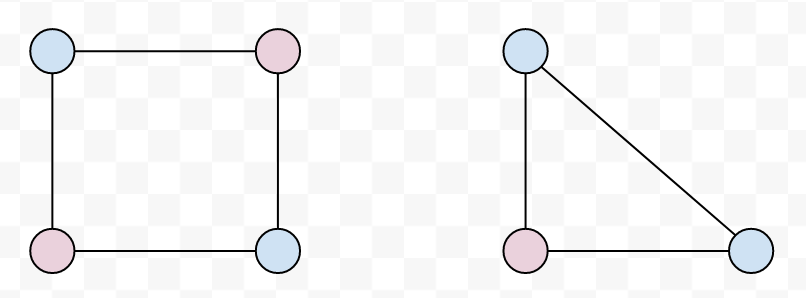
\includegraphics[scale=0.6]{q1.png}
    \caption{Q1}
    \label{fig:my_label}
\end{figure}

Now consider the general case with any subgraph $H$ of $G$ and a contraction between any two nodes, $u, v$, and call the new node $w$. Since $u, v$ are adjacent, they have different colours, $c_1$ and $c_2$ respectively. Any nodes that are adjacent to $u$ must not have colour $c_1$ and vice versa for $v$. \\

After the contraction, there are two cases:
\begin{enumerate}
    \item $w$ is adjacent to a node with colour $c_1$ or $c_2$, and thus the contraction made this graph not $k$-colourable, and thus is no longer minor-closed.
    \item $w$ is adjacent to nodes with colouring NOT in the set $c_1, c_2$ and we contract again. Eventually, we'll reach a state where the graph reaches case 1, and thus is no longer minor-closed.
\end{enumerate}
\end{proof}
\end{problem}

\begin{problem} \underline{Answer:}
\begin{proof}
Let each hexagon be a set of points in $\R^2$ that share the same colour and let a walk from a point to another be the walk of Euclidean length 1. Since we want to arrange colours based on this property, we want to make sure that two hexagons with the same colour are not within walkable distance. \\

Let's consider the middle white hexagon in figure 2. We see that in order to reach any other white hexagon, it must go through at exactly 2 other tiles. Since we don't want a walk to exist between these two tiles, we then know that the diameter of each hexagon, which we will call $d$, should be $\sqrt{2} < d < 1$. We can take any number in that range and set $d$ to it and we will not be able to walk from a hexagon of colour $c_i$ to $c_i$.
\begin{figure}[H]
    \centering
    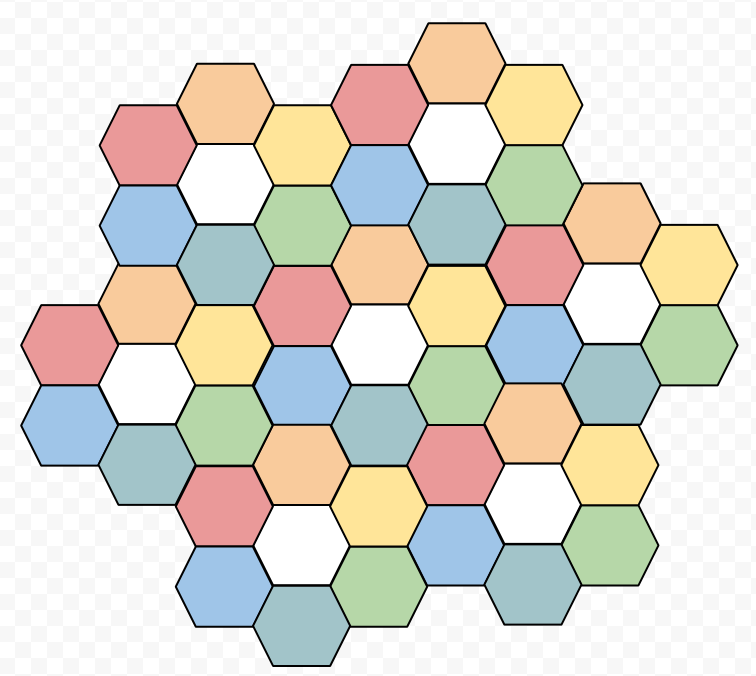
\includegraphics[scale=0.6]{q2.png}
    \caption{Q2}
    \label{fig:my_label}
\end{figure}
\end{proof}
\end{problem}

\begin{problem} \underline{Answer:} This will be proved directly. \\
\begin{proof} 
Now, let's consider the general case for any graph without loops and whose vertices have degree $\leq$ 3. For each vertex, it is adjacent to at most 3 other vertices. In the worst case, we have the complete graph $k_4$, which is 3-regular. $k_4$ is 4-chromatic and therefore is 4-colourable. \\
\end{proof}

Figure 3 is an example of a plane graph without $k_4$ has a subgraph and is 4-chromatic. 
\begin{figure}[H]
    \centering
    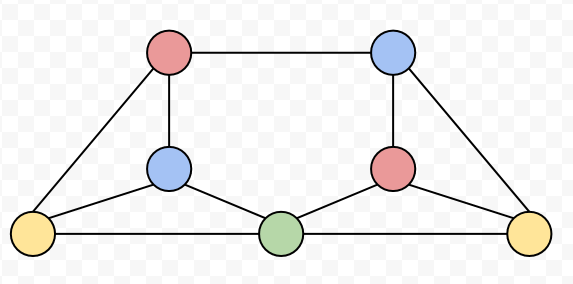
\includegraphics[scale=0.6]{q3.png}
    \caption{Q3}
    \label{fig:my_label}
\end{figure}
\end{problem}

\begin{problem} \underline{Answer:} \\
\begin{proof}
For the first graph, the chromatic polynomial is $k(k - 1)^2(k - 2)^2$. \\

For the second graph, the chromatic polynomial is $k(k - 1)^3(k - 2)$
\begin{figure}[H]
    \centering
    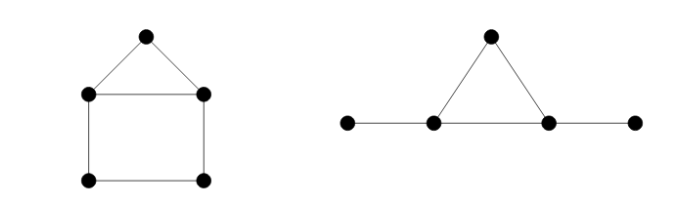
\includegraphics[scale=0.6]{q4.png}
    \caption{Q4}
    \label{fig:my_label}
\end{figure}
\end{proof}
\end{problem}

\begin{problem} \underline{Answer:}
\begin{proof} 
Consider the windmill graph $Wd(n, N)$ and how to construct it. For any windmill graph, there is a central vertex that joins the $N$ $k_n$ graphs. Let's call this vertex $v$. \\

Let's start from $v$ and we see that there are $k$ possible colourings for $v$. \\

Next, let us consider a single connected complete component of $Wd(n, N)$, namely a specific subgraph of $Wd(n, N)$ and let us call this $H$. Since $v$ is a part of $H = (V', E')$ and $H = k_n$, $v$ is adjacent to every other vertex. \\

For all vertices $u \in E'$, we see that it must be adjacent to all other vertices $w \in E'$, and this includes $v$. Remember that $v$ has $k$ colours, and in order for $H$ to be a proper graph colouring, the other vertices in $H$ must have unique colourings. This means that $H$ has a chromatic polynomial of $k(k - 1)(k - 2)...(k - (n - 1)) = k\prod_{i = 1}^{n - 1} (k - i)$. \\

Now consider all $N$ $k_n$ graphs. We can apply the same logic above and arrive at the chromatic polynomial of $Wd(n, N)$. Since the central vertex is shared between all components, we only count it once. Thus, the chromatic polynomial is $k\prod_{i = 1}^{n - 1} (k - i)^N$
\end{proof}
\end{problem}
\end{document}
